\chapter{Introduction}
\label{cha:intro}
My project aims to replicate some of the reinforcement learning algorithms that can be used to play classic Atari 2600 games. It also compares the results of different tests with these algorithms such as varying the hyperparameters of the network. By observing the effects on the trained agents\footnote{Agent. In this case, agent refers to a trained neural network that takes actions in a chosen environment.} when the hyperparameters are changed we can deduce a set of optimal values such that the networks can play three different Atari 2600 games. Overall, the main features of the project are the following:
\begin{itemize}
	\item Agents with raw pixel game data as input, outputting a set of values for the best action.
	\item Agents attempt to find an optimal model of the environment without any prior knowledge.
	\item Visualization of the agents ``brain'' to provide insight into what information the agent is learning.
\end{itemize}

\section{Impact of COVID-19}
COVID-19 has caused widespread disruption across the faculty and University as a whole, and unfortunately it also impacted my plans for the Semester. The circumstances surrounding the pandemic lead to uncertainty around whether it was safe to be at University and made it more difficult to maintain the required level of focus and motivation on the project, mainly as I was concered about if I should travel home or have the possibility of being quarentined in University accomodation. On the otherhand, I know that many people were more affected than I, in compaision my situation was much less disrupted than others.

\section{Motivation}
\label{intro:sec:moti}
Over the past 10 years, there has been significant improvement in the RL (reinforcement learning) algorithms. One reason is that computing power has become cheaply available by using discrete graphics cards. For example, for my project, I used an Nvidia GeForce GTX 1070 that provides 1920 CUDA cores that can be used to accelerate training of neural networks. Despite this, RL algorithms are massively computationally expensive and hence take a long time to train.

Over recent years one of the pioneers in this area is DeepMind, which was acquired by Google in 2014, and they developed the DQN (deep q-network) algorithm in 2013 which they demonstrated could learn directly from the raw pixel data of games to achieve either human-level or super-human level performance.

This research was expanded upon by DeepMind and OpenAI which is based on the original DQN by DeepMind. This research focused on trying to approximate a Q-function and thereby infer the optimal policy. On the other hand, there has recently been a focus on other methods such as A3C and PPO which instead seek to directly optimise in the policy space of the environment.

\section{Objectives}
\label{intro:sec:obj}
Further to what was described in section \ref{cha:intro}, there were a few main objectives of the project. Firstly, I chose three games on which I decided to train the agents, Pong, Breakout, and Space Invaders which are shown below in Figure \ref{fig:atari-screenshot}.

\begin{figure}[htbp]
	\centering
	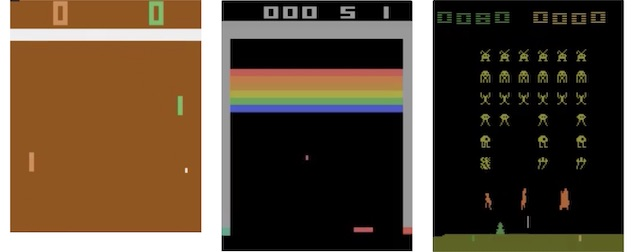
\includegraphics[width=0.7\textwidth]{chapters/chapter1/images/atari-combined.jpg}
	\caption{Screenshots of Pong, Breakout, Space Invaders (left to right).
		\label{fig:atari-screenshot}
	}
\end{figure}


Secondly, I wanted to find a way to explore the internals of a trained agent, to give further insight into what the agent is trying to learn. The reason for this is a researcher could use this information to determine, for example, where the agent has learnt to focus on the frame based on the filter activation maps. Additionally, it also can point towards poor hyperparameter choice such as a high learning rate when the layers have many dead filters. More discussion of these techniques are described in Section \ref{bg:sec:cnn-vis}.

\section{Report structure}
\label{intro:sec:report_struc}

My report is divided into three main sections. First, describing the background of the problem, then going onto giving details of my implementation and finally project evaluations/conclusions.